\documentclass[letterpaper,10pt,onecolumn]{article}

\usepackage{setspace} 
\singlespacing
\usepackage{graphicx}                                        
\usepackage{amssymb}                                         
\usepackage{amsmath}                                         
\usepackage{amsthm}
\usepackage{mathtools}
\usepackage{algorithmic}
\usepackage{url}
\usepackage{tikz}         
\usetikzlibrary{matrix}
\usepackage{listings}
\usepackage{tabu}                             

\newcommand{\tagtree}[3]{#1 \langle #2, #3 \rangle}

\usepackage{geometry}
\geometry{textheight=9.5in, textwidth=7in}
\parindent = 0.0 in
\parskip = 0.1 in
\title{Imperative Programming with Variational Effects}
\author{Alex Grasley}
\begin{document}

\maketitle

\section{Introduction}

At its most basic level, all computation can be viewed as a function from a set of inputs to some
output. For example, consider a function that computes the cost of a car given certain options such
as color, engine size, and warranty. In Haskell we might denote the type of this function as
\texttt{Color -> EngineSize -> Warranty -> Cost}. Given this function, suppose we want to present
a customer with the cost of a car at different warranty levels. We must then run the function a number of
times equal to the number of warranty levels, varying the warranty parameter while keeping the other
parameters constant.

This situation is not ideal. The result is that we repeat work calculating cost based off of color and engine
size every time we try a new warranty variant. Any calculations that are shared across executions are
lost under this model. We would also like a way to explicitly represent in our language what it is 
we are doing when we perform multiple executions and collect the results. That is, we would like a way
to explicitly represent variation as a first-class construct in our language. We can imagine a function
of type \texttt{Color -> EngineSize -> V Warranty -> V Cost} where \texttt{V Warranty} represents a
variational warranty which maps to a variational cost as the result of the function. Because we can
now model variational data explicitly, we can also take advantage of any sharing that occurs between
executions, only branching our execution where we encounter variation.

\section{Background}

\subsection{The choice calculus}

In order to formally represent choices in our programs we employ the choice
calculus \cite{ericthesis,erwig2011choice}. The fundamental unit of the choice calculus is
the \emph{choice}, which is a set of values called \emph{alternatives}.
There are many data structures that can be used to model
choices \cite{walkingshaw2014variational}, so we begin with \emph{tag trees}, one of
the simplest to understand. Tag trees represent the set of alternatives as a binary tree, with concrete
values at the leaves of the tree. We give each node of the tree a name or tag. We call these
tags the \emph{dimensions} of the choices. Notationally we represent these tag trees
via angle brackets. For example, a choice in dimension $A$
between the values $1$ and $2$ is written $\tagtree{A}{1}{2}$. Choices can also be nested inside
each other: $\tagtree{B}{\tagtree{A}{1}{2}}{3}$.

The \emph{selection} operation on a choice eliminates a particular dimension. Each representation
of choices defines a function \emph{sel} that takes a \emph{selector} and a variational value and
eliminates the dimension specified by the selector in the value. For a choice with tag $A$, we represent the
selectors as $A$ and $\neg A$, which select for the left and right alternatives, respectively.
For example, the operation $sel(\neg A, \tagtree{B}{\tagtree{A}{1}{2}}{3})$ produces the
variational value $\tagtree{B}{2}{3}$. Selection is \emph{synchronized} for a given
dimension, meaning that two choices in the same value or expression that share a dimension must always
select the same alternative. For example, in the expression $\tagtree{A}{1}{2}+\tagtree{A}{3}{4}$,
the only possible selections are $1+3$ and $2+4$, while $1+4$ and $2+3$ can never occur due
to synchronization.

We say that a choice is $configured$ when all dimensions
have been eliminated, yielding a plain value without choices. We call these resulting plain values
\emph{variants}. Similar to selection, we define a function \emph{conf} which takes a
\emph{configuration} and a variational value and produces a variant. An easy way to define
configurations for tag trees is as a set of selections for all dimensions. For example, the operation
$conf(\{\neg A,B\}, \tagtree{B}{\tagtree{A}{1}{2}}{3})$ produces the variant $2$.

\subsection{Different choice representations}

Having established tag trees as a simple yet capable representation of choices, we now
examine other data structures that can represent choices. One way of looking at tags
as they are defined above is as boolean variables. Under this view, selection takes a boolean
formula as a selector and checks if that formula implies that a choice's tag is true or false.
If the formula implies that the tag's boolean variable is true, the left alternative is selected;
conversely, if it implies false, then the right alternative is selected.

Tag trees as we have defined them greatly restrict the possible boolean formulas that can act
as selectors and tags. Tags must only be a plain boolean variable and selectors can be either
plain boolean variables or the negation of a boolean variable. If we relax these restrictions by
allowing tags and selectors to be boolean formulas from a proper boolean algebra
consisting of boolean literals, variables, negation, conjunction, and disjunction we achieve a
more expressive form of tag tree that we call \emph{formula trees} \cite{walkingshaw2014projectional,walkingshaw2014variational}.
For an example of formula
trees in action, consider the operation $sel(C \wedge \neg A , A \wedge B \langle 1, 2 \rangle)$,
which produces $2$ because of the implication: $C \wedge \neg A \Rightarrow \neg(A \wedge B)$.

Replacing plain tags with formulas has several advantages. For example, we can simplify tag trees like
$\tagtree{B}{1}{\tagtree{A}{1}{2}}$ to the more compact form $\tagtree{(B \vee A)}{1}{2}$. This is just
one of a number of optimizations that are made possible by representing dimensions as formulas
\cite{walkingshaw2014projectional,hubbard2016formula}. Formula choices are also more convenient
for maintaining a variational context during execution of a program, a fact that will become
more relevant when we present our work on variational imperative programming later in
this work. Despite these advantages over plain tags, formulas incur some cost by introducing boolean
satisfiability problems into many common operations, which is an NP-complete problem. However, thanks to improvements in the
efficiency of modern SAT solvers, often the worst-case NP-complete performance of these satisfiability
problems can be avoided.

While formula trees allow for optimizations that eliminate redundancy found in tag trees,
they still permit the construction of trees with redundant alternatives. If we wish to disallow such
redundancy entirely we use our final choice data structure,
\emph{formula maps} \cite{walkingshaw2014variational}.
A formula map represents choices as a mapping from unique alternatives to formulas, eliminating the
possibility for redundant alternatives. The tag tree $\tagtree{C}{\tagtree{A}{1}{2}}{\tagtree{B}{2}{3}}$
corresponds to the formula map 
$\{1 \Rightarrow A \wedge C, 2 \Rightarrow \neg A \vee B, 3 \Rightarrow \neg B \wedge \neg C\}$.
We require all formula values in the formula map to be disjoint, with their disjoint union as the total
configuration space for the boolean variables contained within it. % how to phrase this?

Formula maps assure us that there is no redundancy, but at the significant cost of maintaining this
invariant when formula maps are created or updated. This requires potentially even more interaction
with satisfiability problems than formula trees. Often it is more advantageous to define a \emph{join}
operation that eliminates redundancy in a formula tree and then to identify the parts of
a variational program that are particularly sensitive to redundancy and insert calls to \emph{join}
at these points.  

\subsection{Properties of choices}

% sharing is desirable. what is sharing?
The choice calculus gives us several desirable properties for variational programs.
The first is \emph{sharing}. A naive approach to executing a variational program is simply to
configure the variational program in order to produce each variant and run them all sequentially.
For a program with $n$ dimensions this results in $2^n$ variants that must be executed. Crucially,
the naive approach must recompute any common elements shared between variants. Embedding
choices in our program, combined with a variability-aware model of execution allows us to exploit this
inherent sharing by only computing shared components once, greatly improving the efficiency of
executing a variational program.

% correctness and the commuting diagram
Another property of choices and variation that we are interested in is \emph{correctness}. In order
to take advantage of the benefits of sharing, we must develop a variability-aware model of execution
that produces variational values as its result. In order to determine whether our variational results
are correct we need a way to relate them back to the individual variants they represent.

Given a function $f : T \rightarrow U$ and its variational counterpart $g : V \rightarrow W$, we say that
the relationship between the two is correct if for some configuration $c$ the following equality holds:
$conf\ c \circ g = f \circ conf\ c$ \cite{hubbard2016formula}. Put simply, configuring the result
of passing a variational value to a variational function should be the same as pre-configuring the input
and the function itself. This can be visualized as the following commuting diagram:

\begin{center}
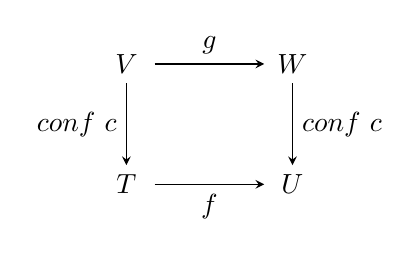
\begin{tikzpicture}
  \matrix (m) [matrix of math nodes,row sep=3em,column sep=4em,minimum width=2em]
  {
     V & W \\
     T & U \\};
  \path[-stealth]
    (m-1-1) edge node [left] {$conf\ c$} (m-2-1)
            edge node [above] {$g$} (m-1-2)
    (m-2-1.east|-m-2-2) edge node [below] {$f$}
             (m-2-2)
    (m-1-2) edge node [right] {$conf\ c$} (m-2-2)
            ;
\end{tikzpicture}
\end{center}

\section{Motivation}

In order to take advantage of the benefits of sharing provided by choices, we must develop variational
models of execution for a given language. We begin by showing that defining variational execution in a pure,
side-effect free evaluation context is a fairly straight-forward exercise before turning to the much more
difficult problem of variational execution with side effects.

\subsection{Pure variational execution}

If we do not have to worry about side effects in our language that we wish to introduce variation to
our task is comparatively easy. We begin by considering a simple arithmetic expression language:

$a ::= n\ |\ a + a\ |\ a * a$

TODO: demonstrate how this works for pure expressions


\subsection{Exceptions}

Exceptions are a common type of effect that proves challenging in a variational setting.
Consider the following program:

\begin{algorithmic}
\STATE $y \coloneqq$ getSecret()
\IF{$y$ is true}
\STATE{\textbf{throw} $e$}
\ENDIF
\STATE{$x \coloneqq$ expensiveFn()}
\end{algorithmic}

In a non-variational context, the behavior of this program should be clear.
If the variable $y$ evaluates to \textbf{true}, then an error is thrown with value
$e$. At this point evaluation should stop, meaning that the variable $x$ is never
assigned in the final statement, avoiding the costly computation of \texttt{expensiveFn}. This effect of halting execution and
returning an error value is the essence of exceptions in non-variational settings.

Now we consider the behavior of the same program in a variational context.
Suppose that the variable $y$ evaluates to the variational value
$A \langle \textbf{true}, \textbf{false} \rangle$. This means that in the left alternative of $A$ we
would evaluate the body of the if statement, while ignoring it otherwise. Therefore,
in the left alternative of $A$ we throw an exception, but otherwise we continue on to the
final statement.

Clearly maintaining the same behavior from the non-variational setting in the variational setting
violates correctness. If we halt execution whenever an exception is
thrown in any variant, then we also stop the evaluation of variants that never encountered an error,
as in our example for the case $\neg A$. Correctness dictates that variants that never encountered
an exception should complete their execution uninhibited.

We also can't simply continue evaluation
in every variant regardless of whether or not we have encountered an error.
Suppose that calling \texttt{expensiveFn} normally would evaluate to the variational value $A\langle 1, 2 \rangle$, but at considerable computational cost in both alternatives.
Because we know that the left alternative of $A$ will ultimately evaluate to the thrown exception $e$, we would
like to avoid the cost involved in computing the value 1 that we will just throw away later, mirroring how throwing an exception short-circuits evaluation in the
non-variational setting. 

Another problem concerns how to keep track of which variants are in error states and what
the error values are. If we want to avoid the cost of pointless evaluation in variants that are in an error
state, we must have some efficient way of determining when evaluation is about to enter such a variant.
In the non-variational context we have no need to store and remember error values during evaluation
because we simply return the error value immediately when it is thrown. In the variational context, we
must now store these values while we continue to evaluate variants that are not in an error state.

\bibliographystyle{plain}
\bibliography{paper}















\end{document}